\chapter{Fock Matrix prediction: A first trial}
\label{chap:fock_matrix_predictions}

SCF methods by nature initially need a density matrix to start off their iterative calculations. Independent of the way the initial guess is chosen the computational effort of this step should be negligible compared to the actual SCF iterations. 
\TODO{Add more details about the Fock matrix prediction - Reasoning for the choice.}

As explained in \autoref{sec:background} (\TODO{Background SCF}) the density matrix $P$ is calculated from the coefficient matrix $C$ which is obtained from the eigenvalue problem of the Fock matrix $F$:
\begin{equation}
    F(P)\,C = SC\varepsilon \rightarrow P = 2CC^T
\end{equation}
Effectively, one performs part of the SCF cycle here to obtain the density matrix, which ideally should be close to the final density matrix. This step takes $\bigO{N^3}$ time, which is assymtotically faster than the $\bigO{N^4}$ time of the SCF cycle. 


\noindent
\begin{figure}[H]
    \centering
    \begin{tikzpicture}[scale=1, every node/.style={transform shape}]

        % Skalierungsfaktor für drei Bilder + Zwischenraum
        \def\imgwidth{0.30\linewidth}

        % Erstes Bild mit Titel
        \node[anchor=south west, inner sep=0] (img1) at (0,0)
            {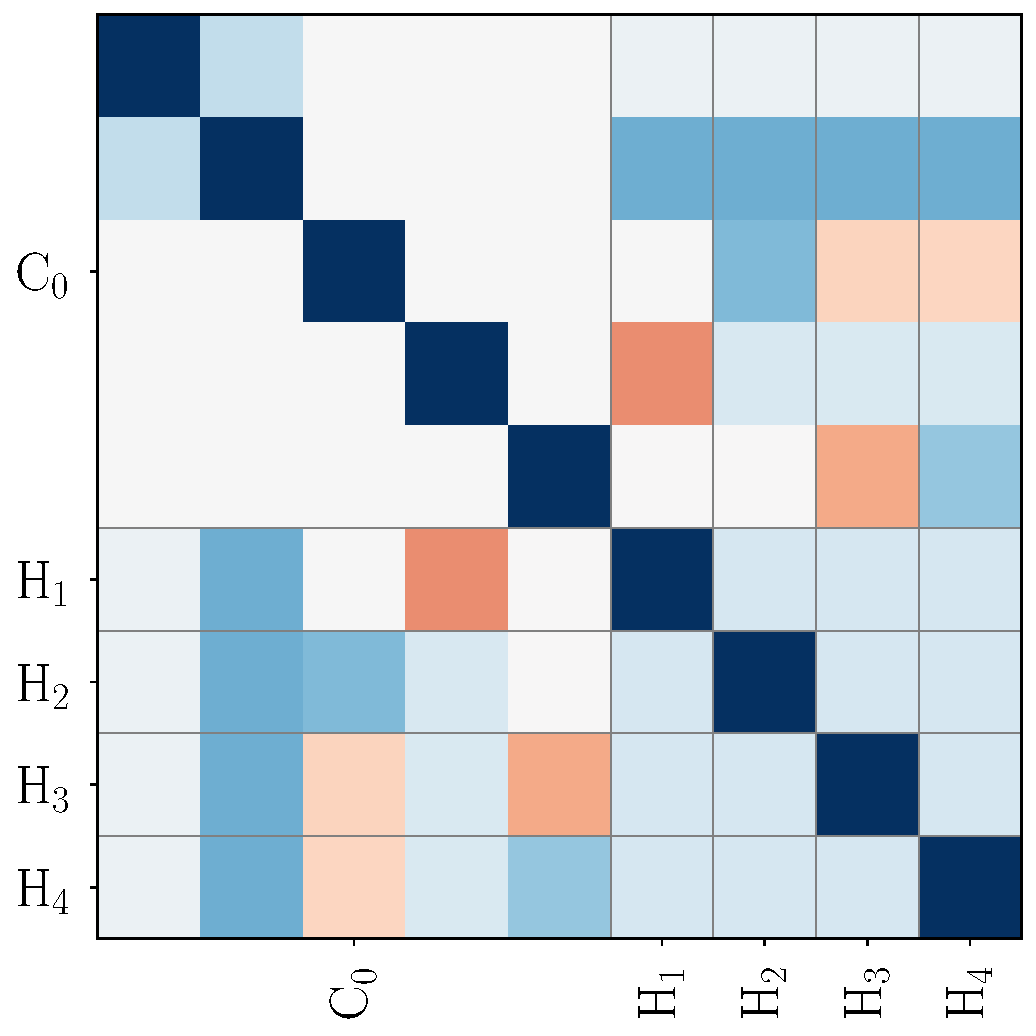
\includegraphics[width=\imgwidth]{../fig/c5h4n2o2/overlap_dsgdb9nsd_000001.pdf}};
        \node[above=2pt of img1.north, anchor=south, font=\small, xshift=10pt] {Overlap};

        % Zweites Bild mit Titel
        \node[anchor=south west, inner sep=0] (img2) at (5.1,0)
            {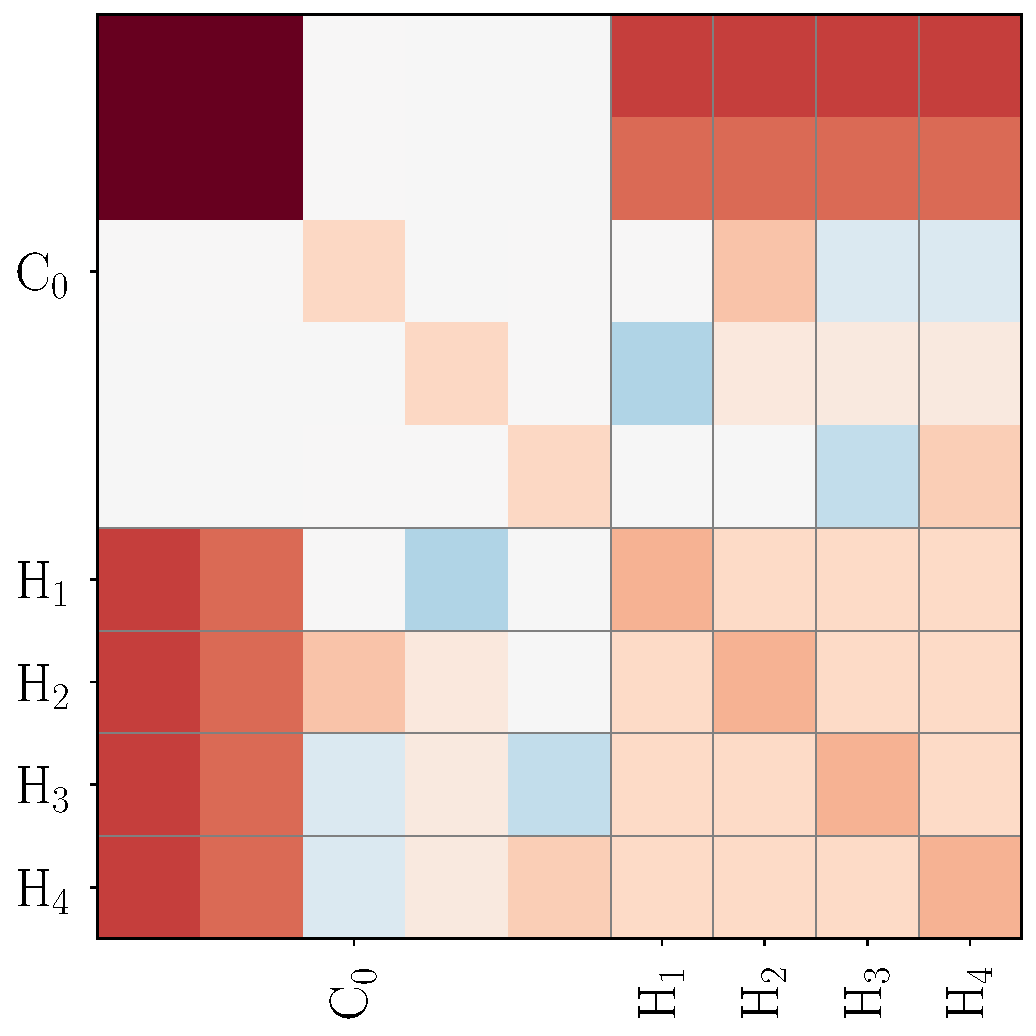
\includegraphics[width=\imgwidth]{../fig/c5h4n2o2/fock_dsgdb9nsd_000001.pdf}};
        \node[above=2pt of img2.north, anchor=south, font=\small, xshift=10pt] {Fock};

        % Drittes Bild mit Titel
        \node[anchor=south west, inner sep=0] (img3) at (10.2,0)
            {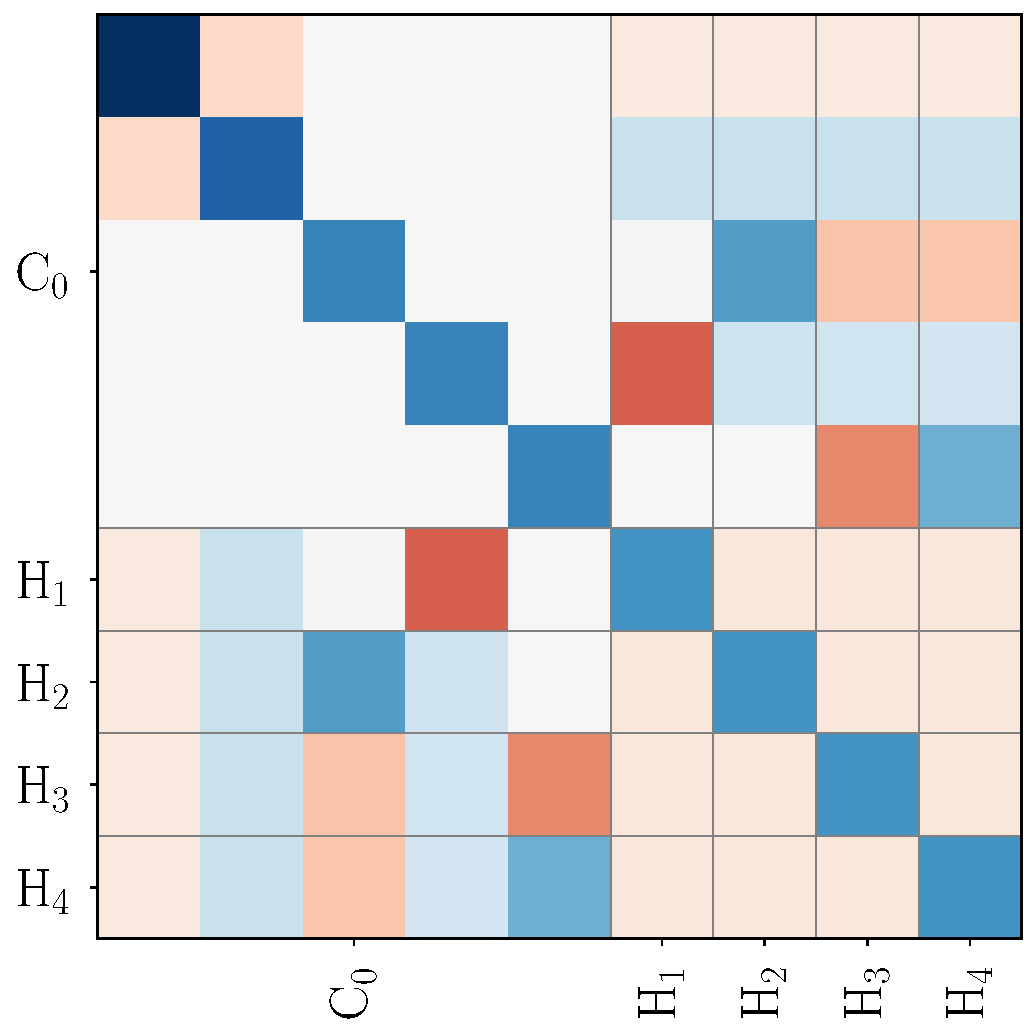
\includegraphics[width=\imgwidth]{../fig/c5h4n2o2/density_dsgdb9nsd_000001.pdf}};
        \node[above=2pt of img3.north, anchor=south, font=\small, xshift=10pt] {Density};
        
        % Pfeil 1: ML model
        \draw[->, thick] (4.7,2.4) -- node[above, align=center, font=\tiny]{ML\\model} (5.2,2.4);

        \draw[->, thick] (9.8,2.4) -- node[above, font=\tiny, yshift=1pt]{$P{=}2CC^{\mathrm{T}}$} (10.3,2.4);
    \end{tikzpicture}
    \caption[Schematic overview data flow]{Schematic overview of the data flow (using \ch{CH4}): overlap matrix to Fock matrix via ML model prediction, and construction of the density matrix from the Fock matrix.}
    \label{fig:method_data_flow}
\end{figure}

The schematic workflow of generating a density matrix from the overlap matrix is shown in \autoref{fig:method_data_flow}. While the overlap and density might look very similar and one might think that predicting the density matrix directly from the overlap matrix would be easier. However, learning the Fock matrix tends to involve fewer strict physical constraints. A Fock matrix primarily needs to be Hermitian, while a density matrix must be strictly positive semidefinite by construction, as well as normalized to the correct number of electrons. That makes direct density matrix learning more challenging, whereas learning the Fock matrix and then obtaining the density through the diagonalization could yield better results. \TODO{Reference?}

\section{\ch{C5H4N2O2}-subset: A first trial}
\label{sec:qm9_c5h4n2o2}

As a proof of concept we will use 508 constitutional isomers\footnote{From the 509 constitutional isomers of \ch{C5H4N2O2} only 508 converged using the sto-3g basis and the B3LYP functional.} of \ch{C5H4N2O2} from the QM9 dataset. 
Single point RKS simulations in \textsc{PySCF} \parencite{ref:pyscf} were performed for these molecules using the B3LYP\footnote{B3LYPG was used to be consitant with the Gaussian} functional and the sto-3g basis. The resulting converged density-, fock-, and overlap-matrices were saved for future training purposes. For our very minimal basis these matrices are of size $49 \times 49$ as can be seen for a converged density in \autoref{fig:density_dsgdb9nsd_022700}. 
Due to the symmetry of the matrices we can discard nearly half of the elements and are left with 1225 features to learn. A rule of thumb for training classical statistical models is to have at least 10 samples per feature. \parencite{ref:rule_of_10} The given dataset of 508 samples is therefore far off from this rule. Keeping this in mind, we will start off our endevaour with a Ridge regression model as a first trial. 

\begin{figure}[H]
    \centering
    \includegraphics[width=\textwidth]{../fig/c5h4n2o2/density\_dsgdb9nsd\_022700.pdf}
    \caption[Density matrix of dsgdb9nsd\_022700 in the sto-3g basis with theory level B3LYP]{Converged density of dsgdb9nsd\_022700 in the sto-3g basis with theory level B3LYP. The density matrix is of size $49 \times 49$ and is symmetric. The diagonal elements are the occupation numbers of the corresponding orbitals.}
    \label{fig:density_dsgdb9nsd_022700}
\end{figure}

\TODO{Switch heading? -> Ridge Regressor as title and not dataset?!}
\textbf{Ridge Regressor model}\\
The Ridge Regressor is setup with a typical $80 / 20$ train/test split. Overlap (input) as well as Fock (output) matrices are flattend and used as is (rescaling did not improve model accuracy). Using a 5-fold cross validation the model is a Multi-Ouput-Regressor is trained using \textsc{scikit-learn} \parencite{ref:sk-learn} with equally $\log_{10}$-spaced $L^2$-regularization parameter $\alpha$ values ranging from $10^{-2}$ to $10^{3}$. Subsequently, the model is retrained with the arithmetic mean of the best performing $\alpha$ values. For the Fock matrix prediction the model yields a RMSE of $0.046$ on the training set and $0.059$ on the test set which indicates slight overfitting. Using the F-Score metric \parencite{ref:Lehtola2019} (outlined in \autoref{subsec:background_cost_function}) \textcolor{red}{which can be used as a proxy for the convergence speed} we obtain the results in \autoref{tab:fscore_comparison} for the model and various guessing schemes impolemented in \textsc{PySCF} (further guessing scheme implementation details can be found in \autoref{sec:pyscf_initial_guessing_methods}).

\begin{table}[h]
    \centering
    \caption{Comparison of different guessing schemes for 102 (20\%) test samples from the \ch{C5H4N2O2} subset from QM9 \parencite{ref:article1_qm9}. The F-score is calculated using the Fock matrix prediction from the Ridge regression model and various guessing schemes implemented in \textsc{PySCF}. The number of iterations until convergence is shown as well as the percentage samples not converging within 50 iterations and the inference time as a factor of the inference time of the minao guess.}
    \label{tab:fscore_comparison}
    \resizebox{\textwidth}{!}{
    \begin{tabular}{l
                    S[table-format=1.2(2)]
                    S[table-format=1.3(3)]
                    S[table-format=1.2(2)]
                    S[table-format=1.3(3)]
                    S[table-format=1.3(3)]
                    S[table-format=1.3(3)]}
        \toprule
        \textbf{Method} & \texttt{Ridge-model} & \texttt{minao} & \texttt{1e} & \texttt{atom} & \texttt{huckel} & \texttt{vsap} \\
        \midrule
        F-score / 1 & 0.88 \pm 0.06 & 0.899 \pm 0.002 & 0.71 \pm 0.02 & 0.802 \pm 0.0010 & 0.840 \pm 0.010 & 0.993 \pm 0.002 \\
        Iterations / 1 & 18 \pm 6 & 11.7 \pm 1.0 & 23 \pm 4 & 11.4 \pm 0.8 & 22 \pm 6 & 12.8 \pm 1.1 \\
        Not-Converged / \% & 15 & 0 &  31 & 0 & 27 & 0\\
        Inference-speed / 1 & 1.8 \pm 0.9 & 1.0 &  0.18 \pm 0.15 & 1.7 \pm 1.4 & 2.0 \pm 1.0 & 8 \pm 5 \\
        \bottomrule
    \end{tabular}
    }
\end{table}
Ridge regression seems to do slightly better than the \texttt{1e} and \texttt{huckel} guessing schemes but drastically worse in comparison to the \texttt{minao}, \texttt{atom} and \texttt{vsap} guessing schemes. Furthermore, it has to be noted that the correlation of the F-score with the number of iterations is not given here. This hints at the fact that some guessing strategies might guess better in regions in the density matrix which are more relevant for convergence speed than others. While \texttt{vsap} yields by far the highest F-score, it on average takes one iteration more to converge than the \texttt{minao} guessing scheme. \\
Comparing the normalized difference to the reference density for the 102 test sample for \texttt{minao}, \texttt{vsap} and the Ridge regression model in \autoref{fig:density_error_comparison} gives different error patterns.  

\begin{figure}[H]
    \centering
    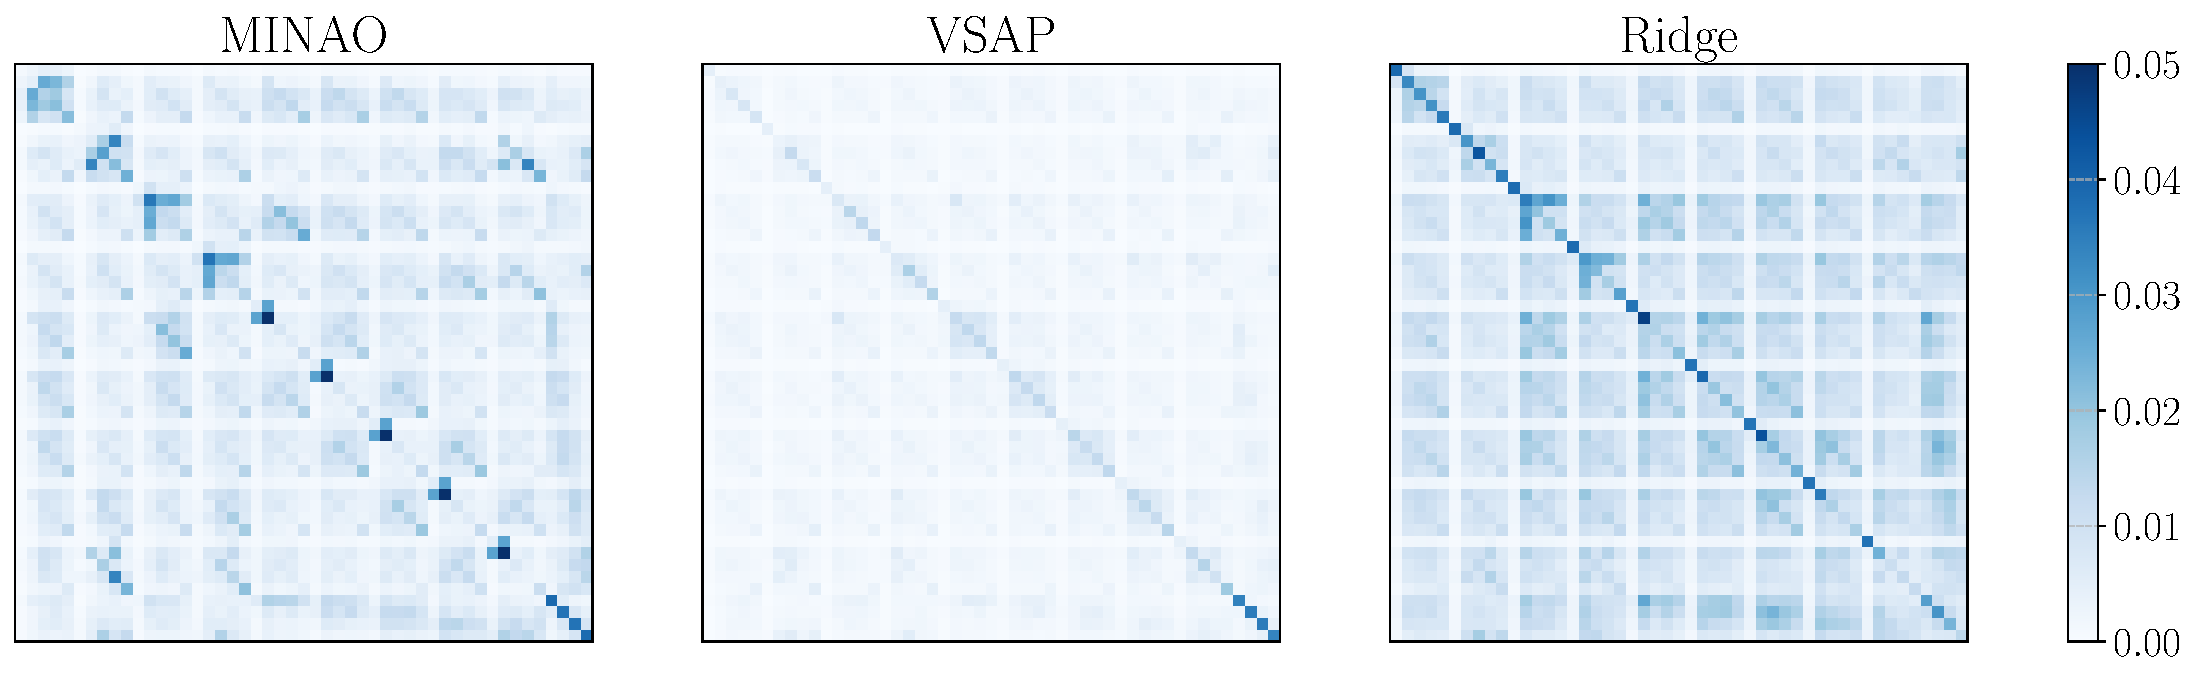
\includegraphics[width=\textwidth]{../fig/c5h4n2o2/density_error_comparison.pdf}
    \caption[Normalized difference of density guesses]{Normalized mean difference of density guesses to converged density for \texttt{minao} \& \texttt{vsap} guess and the Ridge regression model evaluated on the testset: 102 (20\%) test samples from the \ch{C5H4N2O2} subset from QM9 \parencite{ref:article1_qm9}.}
    \label{fig:density_error_comparison}
\end{figure}
All three guessing schemes have spots on the main diagonal of the density matrix where they are likely to differ from the reference solution. Interestingly, a Mullikan population analysis (see \TODO{Background}) \parencite{ref:Mulliken_population_analysis} yields a mean value of $31.766$ the test set prediction for \texttt{minao} while \texttt{vsap} yield the expected $32$ (only $\alpha$-electrons). This slight deviation in the guess doesn't impair the convergence process, as this is fixed anyhow during the first self consistent iteration. Comparing \texttt{minao} and \texttt{vsap} with our Ridge Model the later fares worse on the main diagonal, especially for p-Orbitals. While \texttt{minao} exhibits more pronounced off-diagonal noise, particularly in the top right, this does not significantly affect convergence. These deviations appear to be less detrimental than the smaller diagonal inaccuracies observed in \texttt{vsap}. \\
From that we might conclude that a good guess should be close to the reference density especially on the main diagonal, but not necessarily in the off-diagonal elements. We shall continue to investigate this in the next section.

\section{Predicting the Main Diagonal}
\label{sec:main_diagonal}
\TODO{Reference Cartus + GWH construction}

Ideas: 
\begin{itemize}
    \item Maybe use spectral loss (eigenvalues?!)
    \item CNN
    \item NN 
    \item Maybe two step network -> first guess fock then get rid of noise?
\end{itemize}


\section{Building guesses block-by-block}
\label{sec:blockwise_guessing}
\TODO{Guess main diagonal and then construct or guess off-diagonal elements.}